%%=============================================================================
%% Inleiding
%%=============================================================================

\chapter{\IfLanguageName{dutch}{Inleiding}{Introduction}}%
\label{ch:inleiding}

De inleiding moet de lezer net genoeg informatie verschaffen om het onderwerp te begrijpen en in te zien waarom de onderzoeksvraag de moeite waard is om te onderzoeken. In de inleiding ga je literatuurverwijzingen beperken, zodat de tekst vlot leesbaar blijft. Je kan de inleiding verder onderverdelen in secties als dit de tekst verduidelijkt. Zaken die aan bod kunnen komen in de inleiding~\autocite{Pollefliet2011}:

\begin{itemize}
  \item context, achtergrond
  \item afbakenen van het onderwerp
  \item verantwoording van het onderwerp, methodologie
  \item probleemstelling
  \item onderzoeksdoelstelling
  \item onderzoeksvraag
  \item \ldots
\end{itemize}

\section{\IfLanguageName{dutch}{Probleemstelling}{Problem Statement}}%
\label{sec:probleemstelling}

Uit je probleemstelling moet duidelijk zijn dat je onderzoek een meerwaarde heeft voor een concrete doelgroep. De doelgroep moet goed gedefinieerd en afgelijnd zijn. Doelgroepen als ``bedrijven,'' ``KMO's'', systeembeheerders, enz.~zijn nog te vaag. Als je een lijstje kan maken van de personen/organisaties die een meerwaarde zullen vinden in deze bachelorproef (dit is eigenlijk je steekproefkader), dan is dat een indicatie dat de doelgroep goed gedefinieerd is. Dit kan een enkel bedrijf zijn of zelfs één persoon (je co-promotor/opdrachtgever).

\section{\IfLanguageName{dutch}{Onderzoeksvraag}{Research question}}%
\label{sec:onderzoeksvraag}

Wees zo concreet mogelijk bij het formuleren van je onderzoeksvraag. Een onderzoeksvraag is trouwens iets waar nog niemand op dit moment een antwoord heeft (voor zover je kan nagaan). Het opzoeken van bestaande informatie (bv. ``welke tools bestaan er voor deze toepassing?'') is dus geen onderzoeksvraag. Je kan de onderzoeksvraag verder specifiëren in deelvragen. Bv.~als je onderzoek gaat over performantiemetingen, dan 

\section{\IfLanguageName{dutch}{Onderzoeksdoelstelling}{Research objective}}%
\label{sec:onderzoeksdoelstelling}

Wat is het beoogde resultaat van je bachelorproef? Wat zijn de criteria voor succes? Beschrijf die zo concreet mogelijk. Gaat het bv.\ om een proof-of-concept, een prototype, een verslag met aanbevelingen, een vergelijkende studie, enz.

\section{\IfLanguageName{dutch}{Opzet van deze bachelorproef}{Structure of this bachelor thesis}}%
\label{sec:opzet-bachelorproef}

% Het is gebruikelijk aan het einde van de inleiding een overzicht te
% geven van de opbouw van de rest van de tekst. Deze sectie bevat al een aanzet
% die je kan aanvullen/aanpassen in functie van je eigen tekst.

De rest van deze bachelorproef is als volgt opgebouwd:

In Hoofdstuk~\ref{ch:stand-van-zaken} wordt een overzicht gegeven van de stand van zaken binnen het onderzoeksdomein, op basis van een literatuurstudie.

In Hoofdstuk~\ref{ch:methodologie} wordt de methodologie toegelicht en worden de gebruikte onderzoekstechnieken besproken om een antwoord te kunnen formuleren op de onderzoeksvragen.

% TODO: Vul hier aan voor je eigen hoofstukken, één of twee zinnen per hoofdstuk

In Hoofdstuk~\ref{ch:conclusie}, tenslotte, wordt de conclusie gegeven en een antwoord geformuleerd op de onderzoeksvragen. Daarbij wordt ook een aanzet gegeven voor toekomstig onderzoek binnen dit domein.

------------------------------

\subsection{Probleemstelling}

In de zorgindustrie wordt er steeds meer gesproken over 'alarmmoeheid'. Volgens \textcite{Ferrara2023} kan alarmmoeheid worden omschreven als ''een overprikkeling of zintuiglijke overbelasting, in staat tot het veroorzaken van gevoelloosheid ten opzichte van alarmen door een te groot aantal alarmen die foutief of klinisch onbelangrijk zijn.'' De ernst van de gevolgen van deze moeheid is echter verontrustend. Zo stelt \textcite{Ferrara2023} dat de gedragsmatige reactie van het verplegend personeel, dat lijdt aan een hoge alarmmoeheid, ongepast is. Deze reacties variëren tussen het geluid van het alarmsignaal aanpassen en volledige uitschakeling van het alarm. Wat dus een mogelijk gevaar voor de patiënt inhoudt. Deze stelling wordt bevestigd door het onderzoek van \textcite{Casey2018}. Uit hun onderzoek kwam naar voren dat 90,2 \%, van het geïnterviewde verplegend personeel, oordeelt dat foutieve of klinisch onbelangrijke alarmen frequent voorkomen, de patiëntenzorg verstoren en het vertrouwen in het alarmsysteem beschadigen. Verder zou tot 80,5\%, van het geïnterviewde verplegend personeel, het alarmsysteem soms deactiveren.
\\\\
Twee van de onderdelen van dit alarm-/\\monitoringsysteem zijn het DECT-systeem en het BELET-systeem. Het DECT-systeem is het audiosysteem dat gebruikmaakt van een mobiel toestel om binnen een bedrijf, in deze situatie een ziekenhuis, tussen diensten en personeel te communiceren. Hoewel het systeem al een hele tijd bestaat, sinds 1993, toch zijn er enkele gebreken. Zo is er interferentie met andere medische apparatuur, bedekkingsbeperkingen en de gelimiteerde functionaliteit. De laatste zou een update/upgrade kunnen gebruiken om visuele ondersteuning te bieden aan het personeel.
In tegenstelling tot het DECT-systeem, ligt het BELET-systeem volledig bij de patiënt. Deze is in bezit van een alarmknop waarmee hulp kan worden opgeroepen. Deze alarmsignalen kunnen ook foutief zijn, en zo bijdragen aan de alarmmoeheid.\\

Volgens \textcite{Coiera2006} bestaat de informatie-uitwisseling in gezondheidszorg voornamelijk uit communicatie tussen personen. Dit wordt een ''Communication space'' genoemd. Dit omvat onder andere conversaties over telefoon en in persoon, e-mails, brieven, \ldots . Verder wijst het onderzoek van \textcite{Coiera2006} aan dat de complexiteit van conversaties stijgt naarmate er meer mensen betrokken raken. Dit komt omdat er verschillende conversaties tussen 2 personen kunnen gevoerd worden.

\begin{figure}[h]
  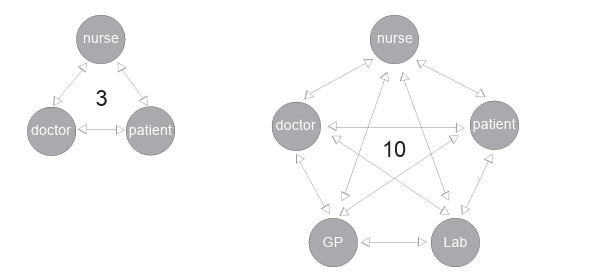
\includegraphics[width=\linewidth]{../graphics/Number-of-conversations.png}
  \caption{Aantal mogelijke conversaties stijgt samen met het aantal personen dat deelneemt aan communicatie. Uit ''Communication Systems in Healthcare'' door \autocite{Coiera2006}}
  \label{fig:aantal conversaties}
\end{figure}

Het is de combinatie van de stijging in complexiteit van informatie uitwisselen met de nadelen van het DECT-systeem en de gevaren van alarmmoeheid die ervoor zorgen dat het huidige systeem wordt in vraag getrokken. Zo bekomen we ook de hoofdvraag die wordt behandeld in deze bachelorproef: \textit{''Hoe kan de informatieuitwisseling tussen artsen en verplegendpersoneel in ziekenhuizen verbeterd worden door het inzetten van nieuwe technologieën''}.\\

Om op deze vraag te antwoorden zullen er verschillende deelvragen moeten worden beantwoord:
\begin{enumerate}
  \item \textit{Wat zijn de kenmerken van het DECT-\\systeem?}
  \item \textit{Wat is het huidige systeem (met \hyphenation{rand-apparatuur}randapparatuur) en wat zijn de nadelen hiervan?}
  \item \textit{Hoe kan een zorgsituatie worden gesimuleerd?}
\end{enumerate}

\subsection{Bachelorproef}
Deze bachelorproef zal focussen op het onderzoeken van welke innovaties een waardevol alternatief kunnen zijn voor het DECT-systeem. Dit onderzoek is gericht op IT-personeel in gezondheidszorginstituten.\\\\

Om een antwoord te formuleren op de hoofdvraag zullen er tussenstappen worden genomen. Deze tussenstappen zijn opgesteld als deelvragen:

\begin{enumerate}
  \item \textit{Welke pogingen zijn al ondernomen om het DECT-systeem als standaard?}
  \item \textit{Wat zijn de minimumvereisten voor technologieën, om als alternatief te kunnen \\worden beschouwd?}
  \item \textit{Welke andere communicatiemogelijkheden zijn er die voldoen aan de minimumvereisten?}
  \item \textit{Welke mogelijke data-integratiemogelijkheden hebben de alternatieven?}
  \item \textit{Welke eigenschappen van het alternatief hebben een vermindering in alarmmoeheid als gevolg?}
  \item \textit{Vanaf wanneer is het haalbaar om te implementeren op economisch vlak?}
\end{enumerate}

De proof of concept die wordt opgesteld tijdens de bachelorproef is in samenwerking met Citymesh en met 360° Zorglab. Citymesh is een bedrijf dat zich specialiseert in connectiviteit, met focus op permanente en tijdelijke netwerkinfrastructuur. Dit door gebruik te maken van WiFi, 0G-, 4G- en 5G-technologieën. \autocite{Citymesh2024} Het 360° Zorglab is een project van HOGENT. De kern van het Zorglab is het creëren van een wisselwerking tussen disciplines enerzijds en tussen onderzoek, dienstverlening en onderwijs anderzijds. Toekomstige gezondheids- en welzijnsmedewerkers kunnen hier in een veilige omgeving niet-technische skills aanleren in een interprofessionele context. \autocite{HOGENT2024} Het doel van deze samenwerking is een snelle wisselwerking te kunnen creëren om zo meerdere malen de testfases te kunnen doorlopen. 
